\documentclass[10pt,letterpaper,unboxed,cm]{article}
\usepackage[margin=1in]{geometry}
\usepackage{graphicx}
\usepackage{enumerate} 
\usepackage{amssymb} 
\usepackage{amsmath}

\newcommand{\st}{~\mid~}
\newcommand{\ind}{$~~~$}
\usepackage{xcolor}

\begin{document}

\hfill{CSE 105 Fall 2025}
\hfill{Homework 1}
\hfill{Due: Monday, October 6 at 11:59pm}

\begin{enumerate}
\item \textbf{Computation of a String on a DFA (Section 1)} \newline 

\emph{Question 1: Trace the computation on input w = abba. 
List the sequence of states visited (including start state) and state whether the input w is
accepted. (refer to the DFA for question 1 in the writeup)} \newline 

\boxed{ABBA \rightarrow $~q_0,q_1,q_0,q_0,q_1$ \newline 
\textbf{\ (The input w will not be accepted as the final state is $q_1$, and not $q_2$)}} \newline

\item \textbf{Drawing a DFA (Section 2)} \newline 

\emph{Question 5: Draw a DFA over the alphabet {0,1} that accepts all strings containing an even number
of 0’s.}

\begin{figure}[h!] % [h!] is a float specifier for placement (here, approximately here)
    \centering % Centers the image
    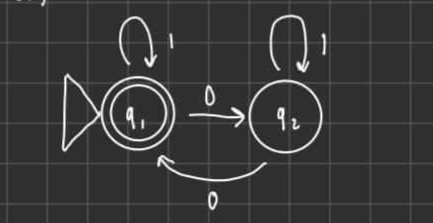
\includegraphics[width=0.75\linewidth]{images/cse105q5.png} % Adjust width as needed
\end{figure}

\item \textbf{Describing what a DFA does (Section 3)} \newline 

\emph{Question 9: Describe in words the set of strings accepted by S.
Give two examples of strings S accepts and two it rejects (Refer to DFA in the writeup for question 9)} \newline 

\textbf{Description:} The set of strings accepted by S includes all strings in the described $\sum$ (refer to writeup) 
that end in "1." \newline 

\textbf{Accepted String Examples: }"01","11" \newline
\textbf{Rejected String Examples: }" ","10" \newline

\pagebreak

\item \textbf{Formal Definition of a DFA (Section 4)} \newline

\emph{Question 13: Given the DFA below, write its 5-tuple $(Q, \Sigma, \delta, q_0, F)$ explicitly. Use a table to define O:} \newline

\textbf{5-tuple:} DFA = ($Q$ = \{$q_1,q_2$\}, $\Sigma$ =\{a,b\}, $\delta$, $q_0=\{q_2\}$, $F$=\{$q_1$\}) \newline 

\textbf{Table to define O: }
\begin{center}
    \begin{tabular}{||c || c c||} 
     \hline
         & \textbf{a} & \textbf{b}\\ [0.5ex] 
     \hline\hline
     \textbf{$q_1$} & $q_1$ & $q_2$\\ 
     \hline
     \textbf{$q_2$} & $q_1$ & $q_2$ \\
    \end{tabular}
    \end{center}
\end{enumerate}

\end{document}